\documentclass[../main.tex]{subfiles}

\graphicspath{{../images/}}

\begin{document}
\pagestyle{fancy}
\lhead{Homework 3}
\chead{Junseo Shin}
\rhead{PHYS 463}

\setcounter{section}{3}

\paragraph{1.} For an idea gas in \emph{two dimensions} confined to an area $A$, determine the multiplicity $\Omega(E)$:
For a 2D particle in a box,
\begin{align*}
    E &= \frac{p}{2m} = \frac{\hbar^2 k^2}{2m}  \\
    \implies k &= \sqrt{\frac{2mE}{\hbar^2}}, \quad dE = \frac{\hbar^2 k dk}{m} \qor dk = \frac{m}{\hbar^2 k} dE
\end{align*}
In $k-$space, the area of a microstate is
\begin{align*}
    k_x k_y = \frac{\pi^2}{L^2} = \frac{\pi^2}{A}
\end{align*}
In the range $k \to k + dk$ the area of the peel is a quarter of the circles circumference times the width of the peel $dk$:
\begin{align*}
    \frac{1}{4} (2\pi k) dk = \frac{\pi k dk}{2} 
\end{align*}
So the multiplicity is
\begin{align*}
    \Omega(k) dk &= \frac{1}{2} \frac{\pi k dk}{\pi^2 / A} = \frac{A}{2\pi} k dk \\
    \Omega(E) dE &= \frac{A}{2\pi} (k) \frac{m}{\hbar^2 k} dE = A \frac{m}{2\pi\hbar^2} dE \\
    \implies \Omega(E) &= A \frac{m}{2\pi\hbar^2}
\end{align*}
so for $N$ particles we have to care for $N!$ permutations:
\begin{align*}
    \boxed{\Omega(E) = \frac{A^N}{N!} \qt(\frac{m}{2\pi\hbar^2})^N}
\end{align*}

\newpage
\paragraph{2.} van der Waals gas
\begin{align*} \tag{1} \label{eq:vdw}
    \qt(p + \frac{a}{v^2})(v - b) = RT
\end{align*}
where $v \equiv V/n$ is the molar volume.
\begin{enumerate}
    \item [(a)] The constant $a$ as units pressure times molar volume squared which captures the long range attractions, or the positive pressure that keep the molecules together. 
    The constant $b$ has units $V/n$, or molar volume, which expressess the occupied volume of the molecules.
    \item [(b)] Molar energy (energy of one mol of gas) dependent on volume:
    To find the dependence of molar energy to volume we start from the first law of thermodynamics
    \begin{align*}
        dE = TdS - pdV \to \frac{dE}{dV} = T\frac{dS}{dV} - p
    \end{align*}
    where we can apply the Maxwell relation
    \begin{align*}
        \pdv{S}{V} = \pdv{p}{T}
    \end{align*}
    so
    \begin{align*}
        \frac{dE}{dV} = T\pdv{p}{T} - p
    \end{align*}
    We can differentiate \eqref{eq:vdw} by $\dv{T}$:
    \begin{align*}
        (v - b) \frac{dp}{dT} = R \implies \pdv{p}{T} = \frac{R}{v - b}
    \end{align*}
    Thus
    \begin{align*}
        \frac{dE}{dV} &= T\frac{R}{v - b} - p 
    \end{align*}
    solving \eqref{eq:vdw} for $p$
    \begin{align*}
        p = \frac{RT}{v - b} - \frac{a}{v^2}
    \end{align*}
    and substituting back into the energy equation
    \begin{align*}
        \frac{dE}{dV} &= T\frac{R}{v - b} - \qt(\frac{RT}{v - b} - \frac{a}{v^2}) \\
        &= \boxed{\frac{a}{v^2}}
    \end{align*}
    \item [(c)] Show that molar heat capacity is independent of volume: Starting with the relation
    \begin{align*}
        c_V = \qt(\frac{\dbar Q}{dT})_V = T \qt(\pdv{S}{T})_V
    \end{align*}
    and differentiating with respect to volume (with $T$ constant)
    \begin{align*}
        \qt(\pdv{c_V}{V})_T &= T \qt[\pdv{V}\qt( \pdv{S}{T})] \\
        &= T \qt[\pdv{T} \pdv{S}{V}]_V \qusing \pdv{S}{V} = \pdv{p}{T} \\
        &= T \pdv[2]{p}{T} = 0
    \end{align*}
    using what we found for $p$ in part (b), So $c_V$ is independent of volume.
    \item [(d)] Taking temp $T$ and volume $v$ as independent parameters, determine $dS$ in terms of $dv$ and $dT$: 
    \begin{align*}
        s = s(v,T)
    \end{align*}
    so the differential is
    \begin{align*}
        ds = \qt(\pdv{s}{T})_V dT + \qt(\pdv{s}{v})_T dv
    \end{align*}
    So using the Maxwell relation and molar heat capacity equations
    \begin{align*}
        \pdv{s}{T} = \frac{c_V}{T} \qand \pdv{s}{v} = \qt(\pdv{p}{T})_V = \frac{R}{v - b}
    \end{align*}
    We get
    \begin{align*}
        \boxed{ds = \frac{c_V}{T} dT + \frac{R}{v - b} dv}
    \end{align*}
\end{enumerate}

\newpage
\paragraph{3.}
\begin{enumerate}
    \item [(a)] Using the ideal gas law for the molar volume $pV = v RT$ 
    \begin{align*}
        p_i V_i^\gamma &= p_f V_f^\gamma \\
        \frac{v R T_i}{V_i} V_i^\gamma &= \frac{v R T_f}{V_f} V_f^\gamma \\
        T_i V_i^{\gamma - 1} &= T_f V_f^{\gamma - 1}
    \end{align*}
    so
    \begin{align*}
        \implies  \boxed{T_f = T_i \qt(\frac{V_i}{V_f})^{\gamma - 1}}
    \end{align*}
    \item [(b)] With constant entropy $\Delta S = 0$:
    \begin{align*}
        \Delta S(T, V; v) &= v \qt(\int_{T_i}^{T_f} \frac{\dbar Q}{T}) = v \qt(\int_{T_i}^{T_f} c_V \frac{dT}{T} + \int_{V_i}^{V_f} \frac{R}{V} dV) = 0 \\
        &= vc_V \ln(\frac{T_f}{T_i}) + vR \ln(\frac{V_f}{V_i}) = 0 \\
        \implies 0 &= \ln \qt[\frac{T_f}{T_i} \qt(\frac{V_f}{V_i})^{R/c_V}]
    \end{align*}
    where $R = c_P - c_V$ so
    \begin{align*}
        \frac{R}{c_V} = \frac{c_P - c_V}{c_V} = \gamma - 1
    \end{align*}
    Exponentiating both sides and using the result above:
    \begin{align*}
        e^0 = \frac{T_f}{T_i} \qt(\frac{V_f}{V_i})^{\gamma - 1} \implies \boxed{T_f = T_i \qt(\frac{V_i}{V_f})^{\gamma - 1}}
    \end{align*}
\end{enumerate}

\newpage
\paragraph{4.} Molar specifc heat at constant volume for a monoatomic ideal gas $c_V = \frac{3}{2} R$. One mole $n = 1$ of gas is subjected to a cyclic quasi-static process:

% fig hw3_4.png
\begin{figure}[ht]
    \centering
    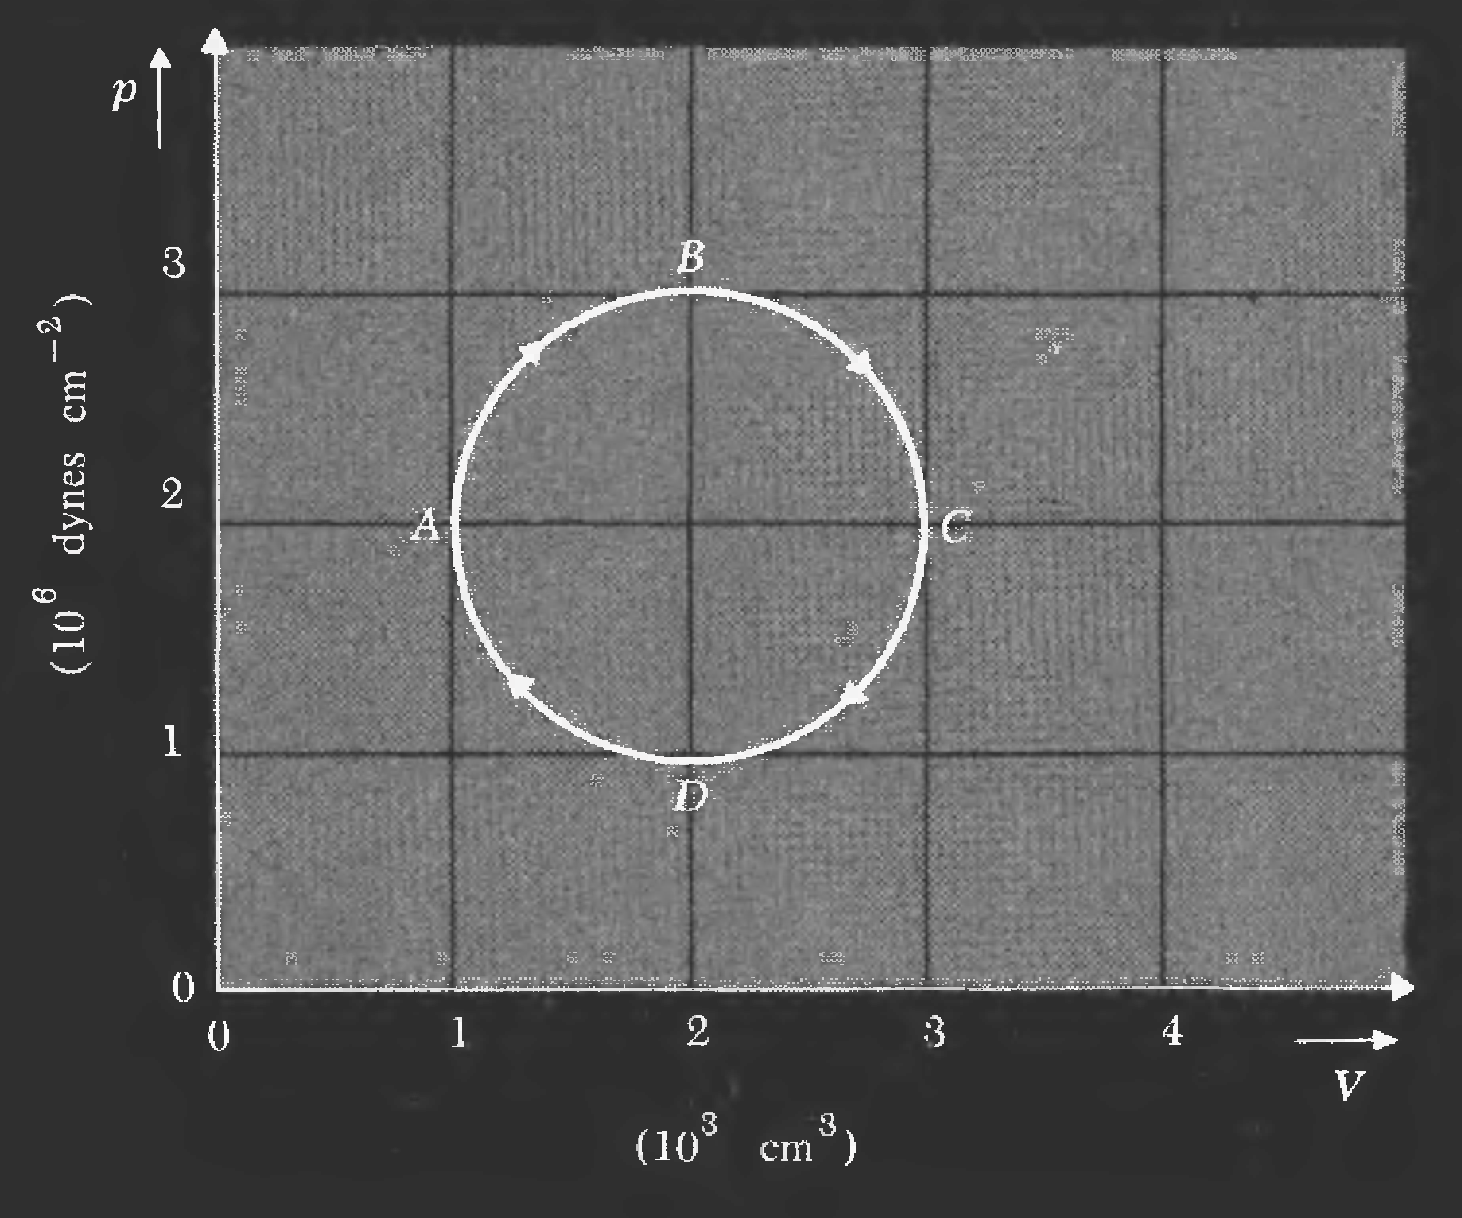
\includegraphics[width=0.5\linewidth]{hw3_4.png}
    \caption{Cyclic process $pV$ diagram}
\end{figure}
\begin{enumerate}
    \item [(a)] The net work in one cycle is the area enclosed by the cycle in the $pV$ diagram i.e. the area of the ellipse $A = \pi pV$:
    \begin{align*}
        W &= \int p dV = \pi \cdot \qty{e6}{dynes.cm^{-2}} \times \qty{e3}{cm^3} \\
        &= \pi \cdot \qty{e9}{dyne.cm} \times \frac{\qty{e-7}{J}}{{\qty{}{dyne.cm}}} \\
        &\approx \boxed{\qty{314}{J}}
    \end{align*}
    \item [(b)] The internal energy difference between state C and A:
    \begin{align*}
        \Delta U &= c_V \delta T \qusing PV = nRT  \implies T = \frac{PV}{R} \\
        &= \frac{3}{2} R \qt(
            \frac{P_C V_C}{R} - \frac{P_A V_A}{R}
        ) \\
        &= \frac{3}{2} \qt(
            P_C V_C - P_A V_A
        ) \quad P_C = P_A = \qty{2e6}{dynes.cm^{-2}} \\
        &= \frac{3}{2} \qt(
            3 - 1 
        ) \times \qty{e9}{dyne.cm} \\
        &= 6 \times \qty{e9}{dyne.cm} \times \frac{\qty{e-7}{J}}{{\qty{}{dyne.cm}}} \\
        &\approx \boxed{\qty{600}{J}}
    \end{align*}
    \item [(c)] The heat absorbed by gas going from A to C via path ABC:
    
    The change in internal energy is the same as (b)
    and the work done is the area under the curve i.e. semicircle $+$  rectangle area:
    \begin{align*}
        Q &= \Delta U + W \\
        &= \qty{600}{J} + [A_\text{rect} + A_\text{semicircle}] \\
        &= \qty{600}{J} + (2 \cdot 2 \qty{e9}{dynes.cm}) + \frac{1}{2} \qty{314}{J} \\
        &= \qty{600}{J} + \qty{400}{J} + \qty{157}{J} \\
        &= \boxed{\qty{1157}{J}}
    \end{align*}
\end{enumerate}

\newpage
\paragraph{5.} The piston is in equilibrium with the force of gravity $+$ the force due to the atmosphere:
\begin{align*}
    F = pA - p_0 A - mg = 0 \implies p = p_0 + \frac{mg}{A} 
\end{align*}
and at equilibrium we can use the adiabatic equation of state $pV^\gamma = \text{constant}$:
\begin{align*}
    pV^\gamma = \qt(p_0 + \frac{mg}{A}) V_0^\gamma = \text{constant}
\end{align*}
where $V = A x$ for the piston moving in the $x$ direction. So we can rewrite Newton's 2nd law as
\begin{align*}
    m \ddot x &= \frac{1}{x^\gamma} \qt(p_0 + \frac{mg}{A}) \qt(\frac{V_0}{A})^\gamma A - mg - p_0 A \\
    &=\frac{1}{x^\gamma} \qt(p_0 + \frac{mg}{A}) \qt(\frac{V_0}{A})^\gamma A - \qt(p_0 + \frac{mg}{A}) A \\ 
    &= \qt(p_0 + \frac{mg}{A}) A \qt[
        \frac{1}{x^\gamma} \qt(\frac{V_0}{A})^\gamma - 1
    ]
\end{align*}
and approximating small $x = x_0 + \delta x = x_0 + \epsilon$ near equilibrium:
\begin{align*}
    x = \frac{V_0}{A} + \epsilon
\end{align*}
We can taylor expand about $x_0$:
\begin{align*}
    \frac{1}{x^\gamma} \approx \frac{1}{(\frac{V_0}{A})^\gamma} - \gamma \frac{\epsilon}{(\frac{V_0}{A})^{\gamma + 1}}
\end{align*}
Substituting back into the equation of motion we now have a function of $\epsilon$:
\begin{align*}
    m \ddot \epsilon &= \qt(p_0 + \frac{mg}{A}) A \qt[
        \frac{\qt(\frac{V_0}{A})^\gamma}{(\frac{V_0}{A})^\gamma} - \gamma \frac{\epsilon \qt(\frac{V_0}{A})^\gamma}{(\frac{V_0}{A})^{\gamma + 1}} - 1
    ] \\
    &= \qt(p_0 + \frac{mg}{A}) A \qt[
        1 - \gamma \epsilon \frac{A}{V_0} - 1
    ] \\
    &= -\qt(p_0 + \frac{mg}{A}) \frac{A^2 \gamma}{V_0}  \epsilon = -k \epsilon
\end{align*}
The solution to the differential equation $m \ddot \epsilon = -k \epsilon$ is a simple harmonic oscillator:
\begin{align*}
    \epsilon = A \cos(\omega t + \phi)
\end{align*}
where we know the angular frequency:
\begin{align*}
    \omega &= 2 \pi \nu = \sqrt{\frac{k}{m}} = \sqrt{\frac{(p_0 + \frac{mg}{A}) \gamma A^2}{mV_0}} \\
    \implies &\boxed{
        \gamma = \frac{4\pi^2 mV_0 \nu^2}{p_0 A^2 + mg A}
    }
\end{align*}

\newpage % 5.10
\paragraph{6.} 
From Reif, the relation between $c_p$ and $c_V$ is
\begin{align*} \tag{5.7.13} 
    c_p - c_V = VT \frac{\alpha^2}{\kappa}
\end{align*}
So the quantity on the right is
\begin{align*}
    VT \frac{\alpha^2}{\kappa} &= \qty{14.72}{cm^3/mol} \times \qty{273}{K} \times
    \frac{\qt(\qty{1.81e-4}{deg^{-1}})^2}{\qty{3.88e-12}{cm^2/dyne}} \times \frac{\qty{1e-7}{J}}{\qty{}{dyne.cm}} \\
    &= \qty{3.39}{J / mol.deg}
\end{align*}
and the specific heat at constant volume is
\begin{align*}
    c_V = c_p - VT \frac{\alpha^2}{\kappa} = \qty{28}{J / mol.deg} - \qty{3.39}{J / mol.deg} = \boxed{\qty{24.6}{J / mol.deg}}
\end{align*}
Furthermore, the ratio is
\begin{align*}
    \gamma = \frac{c_p}{c_V} = \frac{28}{24.6} = \boxed{1.14}
\end{align*}

\newpage % 5.15
\paragraph{7.} For a soap film in Fig. \ref{fig:soap}, the temperature dependence of the surface tension $\sigma$ is given by
\begin{align*}
    \sigma = \sigma_0 - \alpha T
\end{align*}
\begin{figure*}
    \centering
    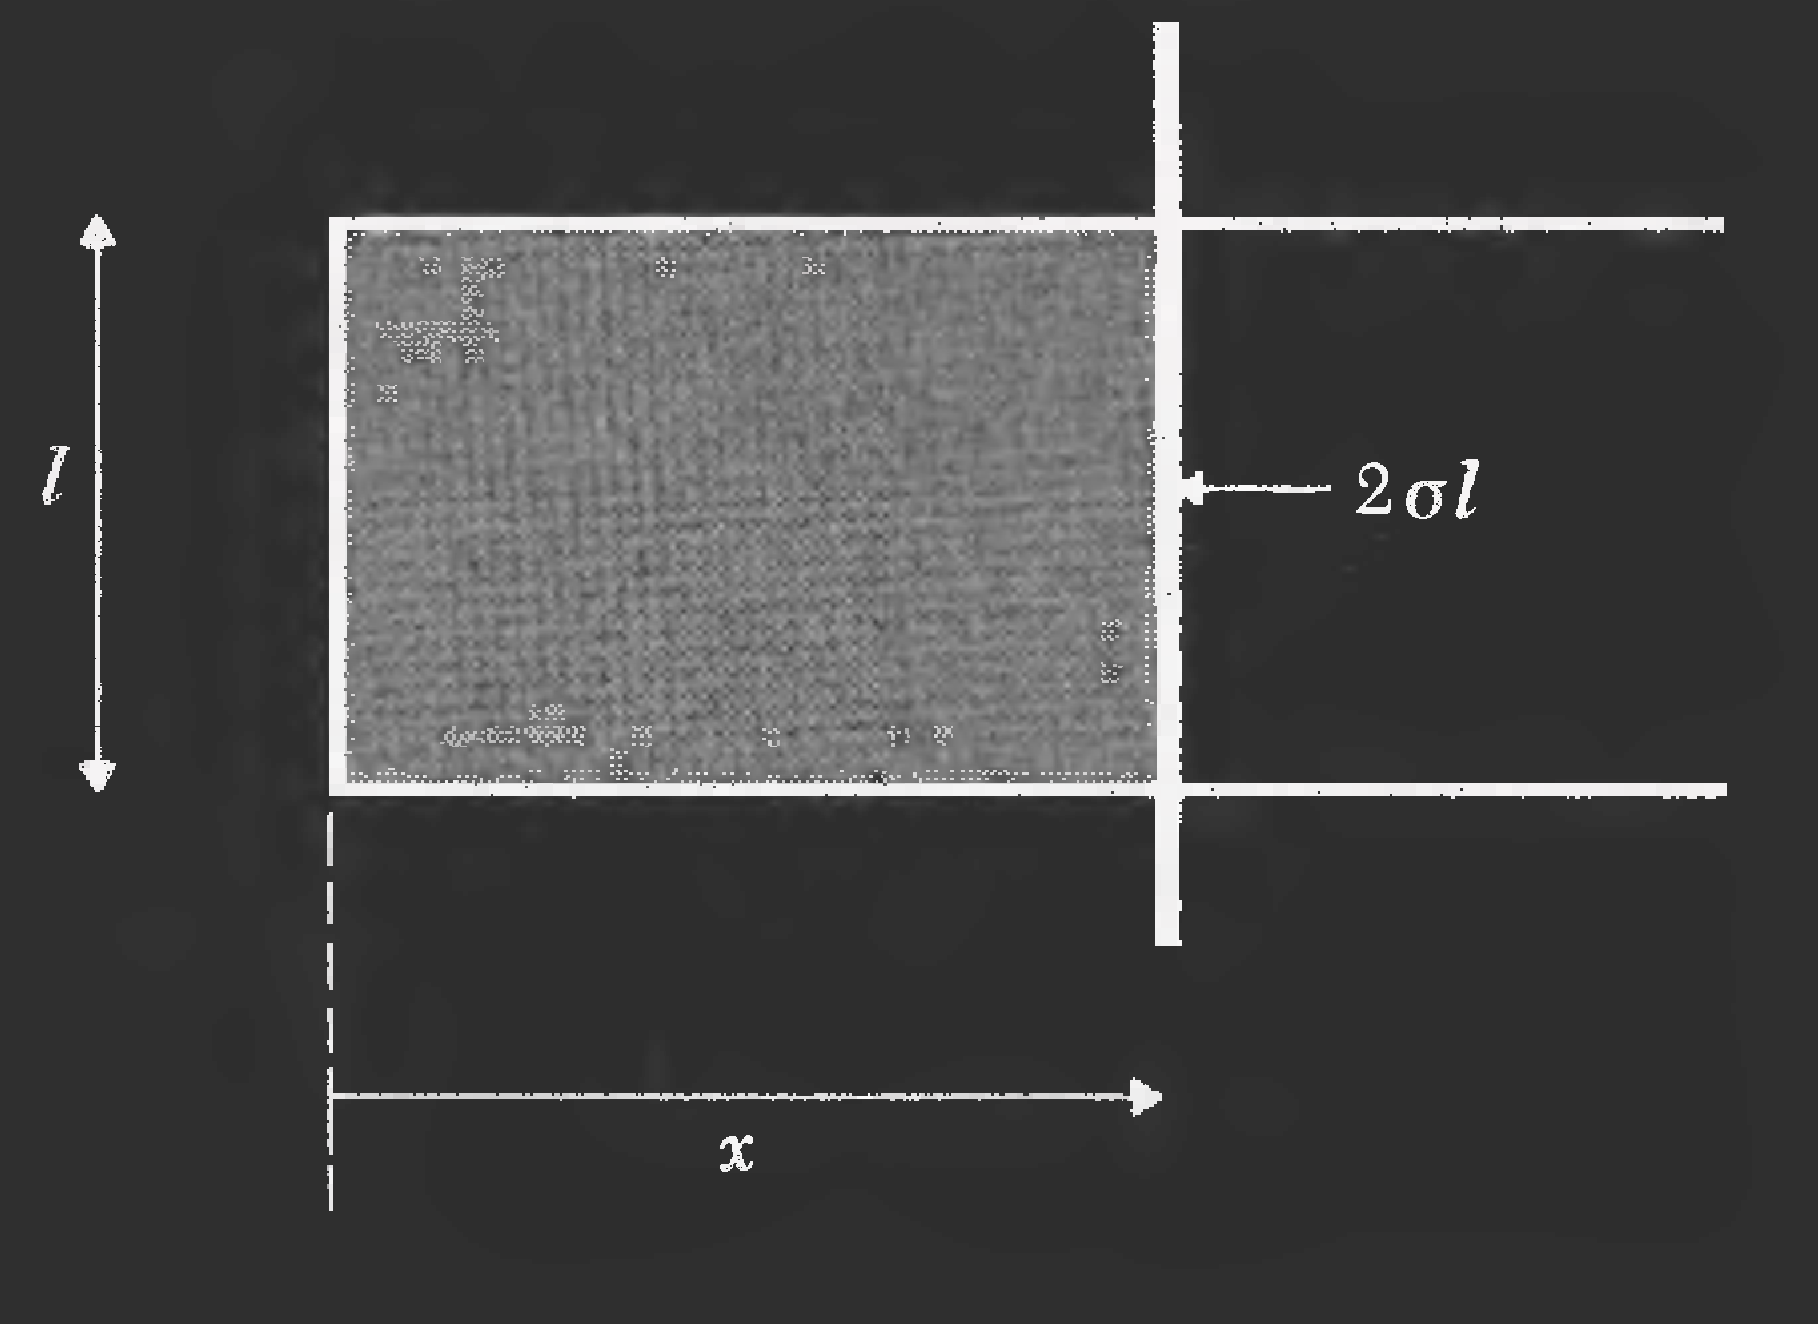
\includegraphics[width=0.6\linewidth]{hw3_7.png}
    \caption{Soap film supported by wire frame with force $2\sigma l$.}
    \label{fig:soap}
\end{figure*}
\begin{enumerate}
    \item [(a)] With $x$ as the only external parameter the change $dE$ in terms of heat $\dbar Q$ absorbed and the work done by it $dx$:
    \begin{align*}
        \dbar Q &= dE + \dbar W, \quad \dbar W = -F dx = -2\sigma l dx \\
        \implies & \boxed{
            dE = \dbar Q + 2\sigma l\; dx
        }
    \end{align*}
    \item [(b)] Calculate the change in mean energy $\Delta E = E(x) - E(0)$ when it is stretched at constant $T_0$ from $x = 0 \to x$:
    \begin{align*}
        \dbar Q &= T dS = dE + \dbar W = dE - F dx \\
        \implies dS &= \frac{dE}{T} - \frac{F dx}{T} = \frac{dE}{T} - \frac{2\sigma l dx}{T}
    \end{align*}
    Using the differential for $S = S(x, T)$ and $E = E(x, T)$:
    \begin{align*}
        dS = \qt(\pdv{S}{T})_x dT + \qt(\pdv{S}{x})_T dx, \qand dE = \qt(\pdv{E}{T})_x dT + \qt(\pdv{E}{x})_T dx
    \end{align*}
    Since the film is stretched at constant $T_0$
    \begin{align*}
        \pdv{S}{T} = 0, \quad \pdv{E}{T} = 0
    \end{align*}
    so
    \begin{align*}
        \qt(\pdv{S}{x})_T dx &= \frac{1}{T} \qt(\pdv{E}{x})_T dx - \frac{2\sigma l}{T} dx \\
        \implies \qt(\pdv{E}{x})_T  &= T \qt(\pdv{S}{x})_T + 2\sigma l
    \end{align*}
    From $T dS = dE - F dx$ we can get the Maxwell relation
    \begin{align*}
        \pdv{S}{x} &= -\pdv{F}{T} = -2l \pdv{\sigma}{T} \qusing \sigma = \sigma_0 - \alpha T \\
        \implies \pdv{S}{x} &= 2l \alpha
    \end{align*}
    Finally
    \begin{align*}
        \qt(\pdv{E}{x})_T &= T \qt(\pdv{S}{x})_T + 2\sigma l = 2l \alpha T + 2l (\sigma_0 - \alpha T) = 2l \sigma_0
    \end{align*}
    so the change in mean energy is
    \begin{align*}
        \Delta E = \int_0^x \qt(\pdv{E}{x})_T dx = \boxed{ 2l \sigma_0 x }
    \end{align*}
    \item [(c)] Calculate the work $W (0 \to x)$ done in order to stretch the film at constant temp from $x = 0 \to x$:
    \begin{align*}
        W = - \int_0^x F dx = - \int_0^x 2\sigma l dx = \boxed{-2l \sigma x} 
    \end{align*}
\end{enumerate}
\end{document}
